\documentclass{book}
\usepackage[shortlabels]{enumitem}
\usepackage{amsmath}
\usepackage{amssymb}
\usepackage{marvosym}
\let\marvosymLightning\Lightning

\usepackage{pgfplots}
\pgfplotsset{compat=newest}
\usepgfplotslibrary{fillbetween}

\newcommand{\mathcolorbox}[2]{\colorbox{#1}{$\displaystyle #2$}}

\newtheorem{definition}{Definition}

\begin{document}

\section {Integralen von Betragsfunktion}
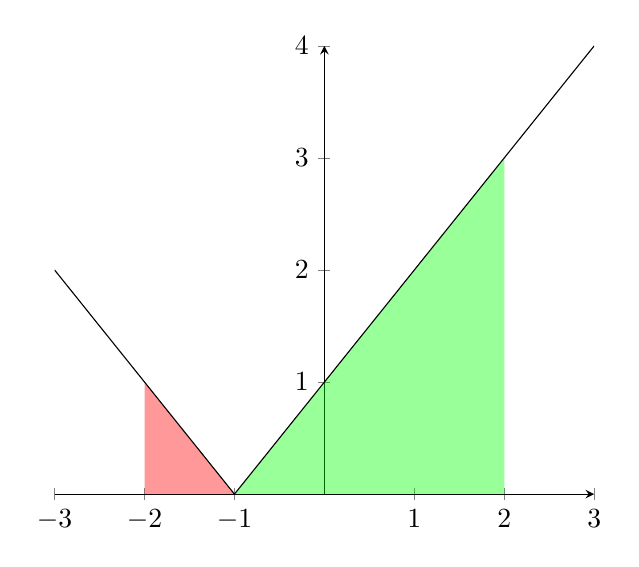
\begin{tikzpicture}
\begin{axis}[axis lines = middle]
\addplot[domain=-3:-1, name path=r]{-x-1};
\addplot[domain=-1:3,name path=g]{x+1};
\path [name path=xaxis]
      (\pgfkeysvalueof{/pgfplots/xmin},0) --
      (\pgfkeysvalueof{/pgfplots/xmax},0);
\addplot[red, opacity=0.4] fill between [of=r and xaxis, soft clip={domain=-2:-1}];
\addplot[green, opacity=0.4] fill between [of=g and xaxis, soft clip={domain=-1:2}];
\end{axis}
\end{tikzpicture}

\[\int_{-2}^2|x+1|dx = \mathcolorbox{pink}{\int_{-2}^{-1}-x-1 dx} + \mathcolorbox{lime}{\int_{-1}^2x+1dx} = [-\frac 12 x^2 - x ]_{-2}^{-1} + [\frac 12 x^2 + x ]_{-1}^{2} \]

andere Beispiel: 
\[\int_{-2}^3 |\frac 12 x|dx = \int_{-2}^0 -\frac 12 x\;dx + \int_0^3 \frac 12 x\;dx\]

\section{Anwendung den Monotonie: Abschätzung des Integrals}
\[\int_1^{100}\frac1{x^2+1}dx\]
\center{es gilt: }
\[\int_1^{100}\frac 1{2x^2}dx\]

????


\section{Uneigentlichen Integralen}
\[\lim_{b\to\infty}\int_a^bf(x)dx\]
\[\lim_{a\to0}\int_a^bf(x)dx\]
\[\dots\]
\raggedright
Beispiele:
\begin{itemize}

\item \[A(b) = \int_1^b \frac 2{x^2} dx = [-\frac 2x]_1^b = -\frac2b + 2\]
\[A = \lim_{b\to\infty}A(b) = \lim_{b\to\infty} -\frac 2b +2 = 2\]
Die Fläche läuft ins Unendliche und troztdem hat einen endlichen Flächeinhalt

\item \[A(b) = \int^b_1 \frac1{\sqrt(x)} dx = [\sqrt x]_1^b = 2\sqrt b - 2\]
\[A = \lim_{b\to\infty}A(b) = \lim{b\to\infty} 2\sqrt b - 2 = \infty \]
Die ins Unendliche reichende Fläche hat keinen endlichen Flächeinhalt

\item
\[A(z) = \int_z^2 \frac 2{\sqrt x}dx = [4 \sqrt x]_z^2 = 4\sqrt 2 - 4\sqrt z\]
\[A = \lim_{z\to 0} (4\sqrt 2 - 4\sqrt z) = \lim_{z\to 0} A(z) = 4\sqrt 2\]
Die ins Unendliche reichende Fläche hat einen endlichen Flächeinhalt

\item \[A(z) = \int_z^2 \frac 1 {x^2} = [-\frac 1x]_z^2 = -\frac 12 + \frac 1 z\]
\[A = \lim_{z\to \infty}-\frac 12 + \frac 1 z = \infty\] 
Die ins Unendliche reichende Fläche hat keinen endlichen Flächeinhalt
\end{itemize}


\end{document}
